\documentclass{standalone}
\usepackage{tikz}
\usetikzlibrary{patterns, positioning}


\begin{document}
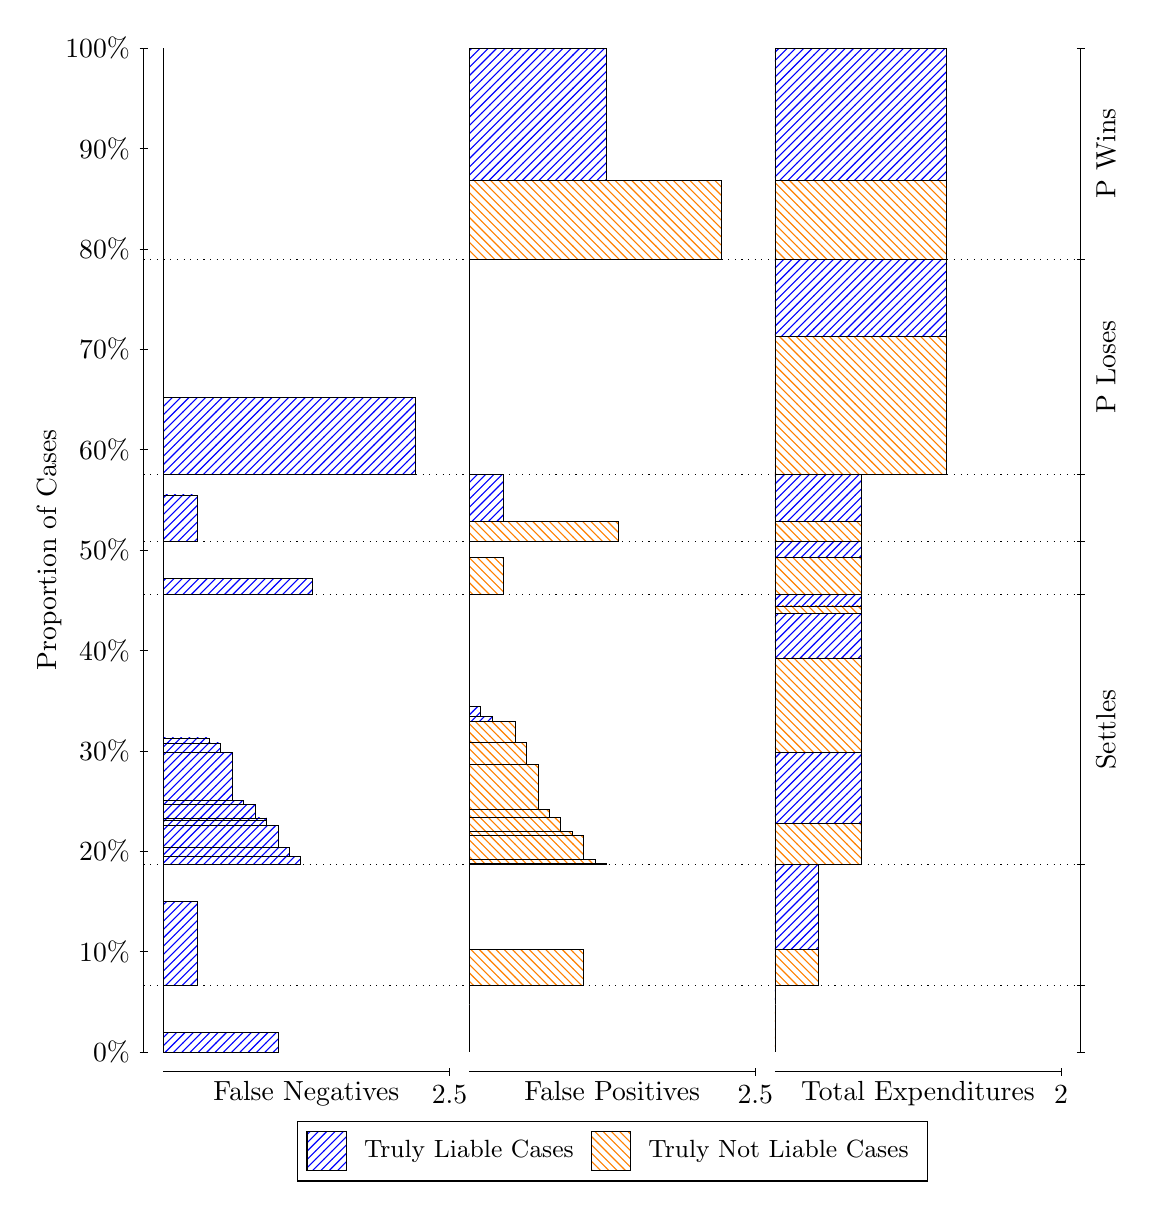
\begin{tikzpicture}
\draw[black, very thin] (1.5,1.75) -- (1.5,14.5);
\node[rotate=90, text=black, anchor=center] at (0.3, 8.125) {Proportion of Cases};
\draw[black, very thin] (1.45,1.75) -- (1.55,1.75);
\node[text=black, anchor=east] at (1.45, 1.75) {0\%};
\draw[black, very thin] (1.45,3.025) -- (1.55,3.025);
\node[text=black, anchor=east] at (1.45, 3.025) {10\%};
\draw[black, very thin] (1.45,4.3) -- (1.55,4.3);
\node[text=black, anchor=east] at (1.45, 4.3) {20\%};
\draw[black, very thin] (1.45,5.575) -- (1.55,5.575);
\node[text=black, anchor=east] at (1.45, 5.575) {30\%};
\draw[black, very thin] (1.45,6.85) -- (1.55,6.85);
\node[text=black, anchor=east] at (1.45, 6.85) {40\%};
\draw[black, very thin] (1.45,8.125) -- (1.55,8.125);
\node[text=black, anchor=east] at (1.45, 8.125) {50\%};
\draw[black, very thin] (1.45,9.4) -- (1.55,9.4);
\node[text=black, anchor=east] at (1.45, 9.4) {60\%};
\draw[black, very thin] (1.45,10.675) -- (1.55,10.675);
\node[text=black, anchor=east] at (1.45, 10.675) {70\%};
\draw[black, very thin] (1.45,11.95) -- (1.55,11.95);
\node[text=black, anchor=east] at (1.45, 11.95) {80\%};
\draw[black, very thin] (1.45,13.225) -- (1.55,13.225);
\node[text=black, anchor=east] at (1.45, 13.225) {90\%};
\draw[black, very thin] (1.45,14.5) -- (1.55,14.5);
\node[text=black, anchor=east] at (1.45, 14.5) {100\%};

\draw[black, very thin] (13.4,1.75) -- (13.4,14.5);
\draw[black, very thin] (13.35,1.75) -- (13.45,1.75);
\node[anchor=west] at (13.35, 1.75) {};
\draw[black, very thin] (13.35,2.5962) -- (13.45,2.5962);
\node[anchor=west] at (13.35, 2.5962) {};
\draw[black, very thin] (13.35,4.1284) -- (13.45,4.1284);
\node[anchor=west] at (13.35, 4.1284) {};
\draw[black, very thin] (13.35,7.5617) -- (13.45,7.5617);
\node[anchor=west] at (13.35, 7.5617) {};
\draw[black, very thin] (13.35,8.2325) -- (13.45,8.2325);
\node[anchor=west] at (13.35, 8.2325) {};
\draw[black, very thin] (13.35,9.0827) -- (13.45,9.0827);
\node[anchor=west] at (13.35, 9.0827) {};
\draw[black, very thin] (13.35,11.818) -- (13.45,11.818);
\node[anchor=west] at (13.35, 11.818) {};
\draw[black, very thin] (13.35,14.5) -- (13.45,14.5);
\node[anchor=west] at (13.35, 14.5) {};

\draw[black, very thin, pattern color=blue, pattern=north east lines] (1.75,1.75) rectangle (3.2033,1.9939);
\draw[black, very thin, pattern color=orange, pattern=north west lines] (1.75,1.9939) rectangle (1.75,2.5962);
\draw[black, very thin, pattern color=blue, pattern=north east lines] (1.75,2.5962) rectangle (2.186,3.667);
\draw[black, very thin, pattern color=orange, pattern=north west lines] (1.75,3.667) rectangle (1.75,4.1284);
\draw[black, very thin, pattern color=blue, pattern=north east lines] (1.75,4.1284) rectangle (3.494,4.2294);
\draw[black, very thin, pattern color=blue, pattern=north east lines] (1.75,4.2294) rectangle (3.3487,4.3451);
\draw[black, very thin, pattern color=blue, pattern=north east lines] (1.75,4.3451) rectangle (3.2033,4.6279);
\draw[black, very thin, pattern color=blue, pattern=north east lines] (1.75,4.6279) rectangle (3.058,4.6902);
\draw[black, very thin, pattern color=blue, pattern=north east lines] (1.75,4.6902) rectangle (3.058,4.7223);
\draw[black, very thin, pattern color=blue, pattern=north east lines] (1.75,4.7223) rectangle (2.9127,4.8897);
\draw[black, very thin, pattern color=blue, pattern=north east lines] (1.75,4.8897) rectangle (2.7673,4.9412);
\draw[black, very thin, pattern color=blue, pattern=north east lines] (1.75,4.9412) rectangle (2.622,5.5499);
\draw[black, very thin, pattern color=blue, pattern=north east lines] (1.75,5.5499) rectangle (2.4767,5.6754);
\draw[black, very thin, pattern color=blue, pattern=north east lines] (1.75,5.6754) rectangle (2.3313,5.7387);
\draw[black, very thin, pattern color=orange, pattern=north west lines] (1.75,5.7387) rectangle (1.75,7.5617);
\draw[black, very thin, pattern color=blue, pattern=north east lines] (1.75,7.5617) rectangle (3.6393,7.7625);
\draw[black, very thin, pattern color=orange, pattern=north west lines] (1.75,7.7625) rectangle (1.75,8.2325);
\draw[black, very thin, pattern color=blue, pattern=north east lines] (1.75,8.2325) rectangle (2.186,8.8257);
\draw[black, very thin, pattern color=orange, pattern=north west lines] (1.75,8.8257) rectangle (1.75,9.0827);
\draw[black, very thin, pattern color=blue, pattern=north east lines] (1.75,9.0827) rectangle (4.9473,10.061);
\draw[black, very thin, pattern color=orange, pattern=north west lines] (1.75,10.061) rectangle (1.75,11.818);
\draw[black, very thin, pattern color=orange, pattern=north west lines] (1.75,11.818) rectangle (1.75,12.822);
\draw[black, very thin, pattern color=blue, pattern=north east lines] (1.75,12.822) rectangle (1.75,14.5);
\draw[black, very thin, pattern color=orange, pattern=north west lines] (5.6333,1.75) rectangle (5.6333,2.3523);
\draw[black, very thin, pattern color=blue, pattern=north east lines] (5.6333,2.3523) rectangle (5.6333,2.5962);
\draw[black, very thin, pattern color=orange, pattern=north west lines] (5.6333,2.5962) rectangle (7.0867,3.0575);
\draw[black, very thin, pattern color=blue, pattern=north east lines] (5.6333,3.0575) rectangle (5.6333,4.1284);
\draw[black, very thin, pattern color=orange, pattern=north west lines] (5.6333,4.1284) rectangle (7.3773,4.1498);
\draw[black, very thin, pattern color=orange, pattern=north west lines] (5.6333,4.1498) rectangle (7.232,4.199);
\draw[black, very thin, pattern color=orange, pattern=north west lines] (5.6333,4.199) rectangle (7.0867,4.5032);
\draw[black, very thin, pattern color=orange, pattern=north west lines] (5.6333,4.5032) rectangle (6.9413,4.5542);
\draw[black, very thin, pattern color=orange, pattern=north west lines] (5.6333,4.5542) rectangle (6.796,4.7287);
\draw[black, very thin, pattern color=orange, pattern=north west lines] (5.6333,4.7287) rectangle (6.6507,4.8328);
\draw[black, very thin, pattern color=orange, pattern=north west lines] (5.6333,4.8328) rectangle (6.5053,5.4015);
\draw[black, very thin, pattern color=orange, pattern=north west lines] (5.6333,5.4015) rectangle (6.36,5.6818);
\draw[black, very thin, pattern color=orange, pattern=north west lines] (5.6333,5.6818) rectangle (6.2147,5.9514);
\draw[black, very thin, pattern color=blue, pattern=north east lines] (5.6333,5.9514) rectangle (5.924,6.0147);
\draw[black, very thin, pattern color=blue, pattern=north east lines] (5.6333,6.0147) rectangle (5.7787,6.1402);
\draw[black, very thin, pattern color=blue, pattern=north east lines] (5.6333,6.1402) rectangle (5.6333,7.5617);
\draw[black, very thin, pattern color=orange, pattern=north west lines] (5.6333,7.5617) rectangle (6.0693,8.0318);
\draw[black, very thin, pattern color=blue, pattern=north east lines] (5.6333,8.0318) rectangle (5.6333,8.2325);
\draw[black, very thin, pattern color=orange, pattern=north west lines] (5.6333,8.2325) rectangle (7.5227,8.4896);
\draw[black, very thin, pattern color=blue, pattern=north east lines] (5.6333,8.4896) rectangle (6.0693,9.0827);
\draw[black, very thin, pattern color=orange, pattern=north west lines] (5.6333,9.0827) rectangle (5.6333,10.84);
\draw[black, very thin, pattern color=blue, pattern=north east lines] (5.6333,10.84) rectangle (5.6333,11.818);
\draw[black, very thin, pattern color=orange, pattern=north west lines] (5.6333,11.818) rectangle (8.8307,12.822);
\draw[black, very thin, pattern color=blue, pattern=north east lines] (5.6333,12.822) rectangle (7.3773,14.5);
\draw[black, very thin, pattern color=orange, pattern=north west lines] (9.5167,1.75) rectangle (9.5167,2.3523);
\draw[black, very thin, pattern color=blue, pattern=north east lines] (9.5167,2.3523) rectangle (9.5167,2.5962);
\draw[black, very thin, pattern color=orange, pattern=north west lines] (9.5167,2.5962) rectangle (10.062,3.0575);
\draw[black, very thin, pattern color=blue, pattern=north east lines] (9.5167,3.0575) rectangle (10.062,4.1284);
\draw[black, very thin, pattern color=orange, pattern=north west lines] (9.5167,4.1284) rectangle (10.607,4.6562);
\draw[black, very thin, pattern color=blue, pattern=north east lines] (9.5167,4.6562) rectangle (10.607,5.5578);
\draw[black, very thin, pattern color=orange, pattern=north west lines] (9.5167,5.5578) rectangle (10.607,6.7544);
\draw[black, very thin, pattern color=blue, pattern=north east lines] (9.5167,6.7544) rectangle (10.607,7.3162);
\draw[black, very thin, pattern color=orange, pattern=north west lines] (9.5167,7.3162) rectangle (10.607,7.4148);
\draw[black, very thin, pattern color=blue, pattern=north east lines] (9.5167,7.4148) rectangle (10.607,7.5617);
\draw[black, very thin, pattern color=orange, pattern=north west lines] (9.5167,7.5617) rectangle (10.607,8.0318);
\draw[black, very thin, pattern color=blue, pattern=north east lines] (9.5167,8.0318) rectangle (10.607,8.2325);
\draw[black, very thin, pattern color=orange, pattern=north west lines] (9.5167,8.2325) rectangle (10.607,8.4896);
\draw[black, very thin, pattern color=blue, pattern=north east lines] (9.5167,8.4896) rectangle (10.607,9.0827);
\draw[black, very thin, pattern color=orange, pattern=north west lines] (9.5167,9.0827) rectangle (11.697,10.84);
\draw[black, very thin, pattern color=blue, pattern=north east lines] (9.5167,10.84) rectangle (11.697,11.818);
\draw[black, very thin, pattern color=orange, pattern=north west lines] (9.5167,11.818) rectangle (11.697,12.822);
\draw[black, very thin, pattern color=blue, pattern=north east lines] (9.5167,12.822) rectangle (11.697,14.5);
\draw[black, dotted] (1.5,2.5962) -- (13.4,2.5962);
\draw[black, dotted] (1.5,4.1284) -- (13.4,4.1284);
\draw[black, dotted] (1.5,7.5617) -- (13.4,7.5617);
\draw[black, dotted] (1.5,8.2325) -- (13.4,8.2325);
\draw[black, dotted] (1.5,9.0827) -- (13.4,9.0827);
\draw[black, dotted] (1.5,11.818) -- (13.4,11.818);
\draw[black, very thin] (1.75,1.5) -- (5.3833,1.5);
\node[text=black, anchor=north] at (3.5667, 1.5) {False Negatives};
\draw[black, very thin] (5.3833,1.45) -- (5.3833,1.55);
\node[text=black, anchor=north] at (5.3833, 1.45) {2.5};

\draw[black, very thin] (5.6333,1.5) -- (9.2667,1.5);
\node[text=black, anchor=north] at (7.45, 1.5) {False Positives};
\draw[black, very thin] (9.2667,1.45) -- (9.2667,1.55);
\node[text=black, anchor=north] at (9.2667, 1.45) {2.5};

\draw[black, very thin] (9.5167,1.5) -- (13.15,1.5);
\node[text=black, anchor=north] at (11.333, 1.5) {Total Expenditures};
\draw[black, very thin] (13.15,1.45) -- (13.15,1.55);
\node[text=black, anchor=north] at (13.15, 1.45) {2};



\node[text=black, centered, rotate=90] at (13.72, 5.8451) {Settles};


\node[text=black, centered, rotate=90] at (13.72, 10.45) {P Loses};
\node[text=black, centered, rotate=90] at (13.72, 13.159) {P Wins};

\draw (7.449999999999999,1.5) node[draw=none] (baseCoordinate) {};
\begin{scope}[align=center]
        \matrix[scale=0.5, draw=black, below=0.5cm of baseCoordinate, nodes={draw}, column sep=0.1cm]{
            \node[rectangle, draw, minimum width=0.5cm, minimum height=0.5cm, pattern color=blue, pattern=north east lines] {}; &
            \node[draw=none, font=\small, text=black] (B) {Truly Liable Cases}; &
            \node[rectangle, draw, minimum width=0.5cm, minimum height=0.5cm, pattern color=orange, pattern=north west lines] {}; &
            \node[draw=none, font=\small, text=black] (B) {Truly Not Liable Cases}; \\
            };
\end{scope}

\end{tikzpicture}
\end{document}